
\tikzset{every picture/.style={line width=0.75pt}} %set default line width to 0.75pt        
\marginnote{
	\begin{minipage}{5.5cm}
		\begin{figure}[H]\centering
			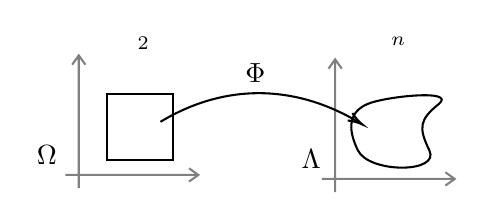
\begin{tikzpicture}[x=0.6pt,y=0.6pt,yscale=-1,xscale=1,scale=.80]
			%uncomment if require: \path (0,237); %set diagram left start at 0, and has height of 237
			
			%Shape: Axis 2D [id:dp3785820715688062] 
			\draw [color={rgb, 255:red, 128; green, 128; blue, 128 }  ,draw opacity=1 ] (50,168) -- (150,168)(60,78) -- (60,178) (143,163) -- (150,168) -- (143,173) (55,85) -- (60,78) -- (65,85)  ;
			%Shape: Axis 2D [id:dp47611229523996135] 
			\draw [color={rgb, 255:red, 128; green, 128; blue, 128 }  ,draw opacity=1 ] (243,171) -- (343,171)(253,81) -- (253,181) (336,166) -- (343,171) -- (336,176) (248,88) -- (253,81) -- (258,88)  ;
			%Shape: Square [id:dp6078316056685962] 
			\draw   (81,107) -- (131,107) -- (131,157) -- (81,157) -- cycle ;
			%Curve Lines [id:da3192192248631224] 
			\draw    (121.5,128) .. controls (172.49,97.31) and (225.92,100.92) .. (272.1,129.14) ;
			\draw [shift={(273.5,130)}, rotate = 211.95] [color={rgb, 255:red, 0; green, 0; blue, 0 }  ][line width=0.75]    (10.93,-3.29) .. controls (6.95,-1.4) and (3.31,-0.3) .. (0,0) .. controls (3.31,0.3) and (6.95,1.4) .. (10.93,3.29)   ;
			
			%Shape: Regular Polygon [id:dp6479810872135613] 
			\draw   (277.12,114.69) .. controls (290.25,108.9) and (345.22,103.1) .. (330.93,114.69) .. controls (316.63,126.28) and (315.46,132.08) .. (323.91,149.46) .. controls (332.36,166.85) and (278.55,166.85) .. (270.1,149.46) .. controls (261.65,132.08) and (263.99,120.49) .. (277.12,114.69) -- cycle ;
			
			% Text Node
			\draw (109,73) node   {$\R^2$};
			% Text Node
			\draw (301,71) node   {$\R^n$};
			% Text Node
			\draw (36,153) node   {$\Omega $};
			% Text Node
			\draw (235,156) node   {$\Lambda $};
			% Text Node
			\draw (193,91) node   {$\Phi $};
			
			
			\end{tikzpicture}
			\caption{Mapeo de una parametrización.}\label{ch0d1}
		\end{figure}
\end{minipage}}